\documentclass[12pt,a4paper]{article}

\usepackage[utf8]{inputenc}
\usepackage[T2A]{fontenc}
\usepackage[ukrainian]{babel}

\usepackage{geometry}
\geometry{left=2cm,right=2cm,top=2cm,bottom=2cm}

\usepackage{graphicx}
\usepackage{placeins}
\usepackage{array,multirow}
\usepackage{booktabs}
\usepackage{caption}
\renewcommand{\thetable}{№\arabic{table}}
\captionsetup[table]{name=Таблиця}

\usepackage{amsmath}
\usepackage{pdflscape}
\usepackage{xcolor}

\usepackage{hyperref}

\begin{document}

    \begin{titlepage}

        % Картинка шапки (по центру, з відступом від верху)
        \begin{center}
\includegraphics[width=0.7\textwidth]{../../../TITLES/letterhead.png}\end{center}

        \begin{center}
            \large Національний технічний університет України\\
            «Київський політехнічний інститут імені Ігоря Сікорського»\\[1em]
            Факультет інформатики та обчислювальної техніки\\
            Кафедра обчислювальної техніки
        \end{center}

        \vfill

        \begin{center}
            \textbf{\LARGE Практична електроніка}\\[2em]
            \textbf{\Large Лабораторна робота №5}\\[1em]
            «Дослідження імпульсних тригерів, аналогових компараторів та схем формування рівнів»
        \end{center}

        \vfill

        \begin{flushright}
            Виконав: студент 2 курсу ФІОТ, гр. ІО-41\\
            \textit{Давидчук А.~М.}\\[1em]
            Перевірив: \textit{Гайдай А.~Р.}
        \end{flushright}

        \vfill

        \begin{center}Київ --- 2025\end{center}

    \end{titlepage}

    % Основний документ:

    \setlength{\parindent}{0em}

    \textbf{\underline{Тема:}} «Дослідження мультивібраторів та генераторів лінійно змінюваної
напруги (ГЛЗН).».
    
    \vspace{1em}

    \textbf{\underline{Мета:}} Дослідити принцип дії, основні властивості та характеристики
мультивібраторів та ГЛЗН.
Ознайомитись із основними параметрами та характеристиками цих пристроїв
та областю їх застосування.

    \begin{center} \textbf{\Large Практична частина} \end{center}

    \setlength{\parindent}{1.5em}

    \begin{center} \textbf{\large Аналіз схеми №1} \end{center}

    \begin{figure}[h!]
        \renewcommand{\thefigure}{\arabic{figure}}
        \centering
        \includegraphics[width=0.4\textwidth]{scheme1.pdf}
        \caption{\centering Схема автоколивального мультивібратора}
    \end{figure}

    \begin{figure}[h!]
        \renewcommand{\thefigure}{\arabic{figure}} % робимо "3.1", "3.2" і т.д.
        \centering
        
\includegraphics[width=0.61\textwidth]{1.png}
        \caption{Часові діаграми роботи схеми}
    \end{figure}

    Шпаруватість імпульсів в цьому прикладі: Q $\approx$ 2.
Згідно цих формул, тривалості імпульсів розраховуються як $T = R \cdot C_1 \cdot \ln\!\left(\frac{1+\beta}{1-\beta}\right)$, де $\beta = R_2/(R_1+R_2)$.

Для $R_1=10 \text{ кОм}$ та $R_2=5 \text{ кОм}$ маємо $\beta = 5/(10+5) = 1/3$.

Тривалість додатного та від’ємного імпульсів залежить від швидкості заряду конденсатора (для 6-го варіанту $C_1 = 6 \text{ мкФ}$) і від значення напруги $U_{\text{н}}$:

\[
t_{\text{ІМ}} = (20 \cdot 10^3) \cdot (6 \cdot 10^{-6}) \cdot \ln(2) \approx 83{,}17 \text{ мc,}
\]
\[
t_{\text{П}} = (10 \cdot 10^3) \cdot (6 \cdot 10^{-6}) \cdot \ln(2) \approx 41{,}58 \text{ мc.}
\]

Розрахунок напруг $U_{\text{н}}$:

\[
U_{\text{н1}} = \frac{R_2}{R_1 + R_2} \cdot U_{\text{нас1}} = \frac{5}{10 + 5} \cdot 13.6 = 4{,}53 \text{ В,}
\]
\[
U_{\text{н2}} = \frac{R_2}{R_1 + R_2} \cdot U_{\text{нас2}} = \frac{5}{10 + 5} \cdot (-13.6) = -4{,}53 \text{ В.}
\]

    З цих формул видно, що розглянута схема дозволяє змінювати шпаруватість вихідних імпульсів.

    \begin{center} \textbf{\large Аналіз схеми №2} \end{center}

    \begin{figure}[h!]
        \renewcommand{\thefigure}{\arabic{figure}} % робимо "3.1", "3.2" і т.д.
        \centering
        \includegraphics[width=0.3\textwidth]{scheme2.pdf}:
        \caption{\centering Схема автоколивального мультивібратора зі шпаруватістю 2}
    \end{figure}

    \begin{figure}[h!]
        \renewcommand{\thefigure}{\arabic{figure}} % робимо "3.1", "3.2" і т.д.
        \centering
        
\includegraphics[width=0.5\textwidth]{2.png}
        \caption{Часові діаграми роботи схеми}
    \end{figure}

    У цій схемі автоколивального мультивібратора відсутні діоди, а резистори 
    $R_2$ та $R_3$ утворюють симетричний подільник напруги. Через це процеси 
    заряджання і розряджання конденсатора $C_1$ мають однакову тривалість, а 
    вихідний сигнал містить прямокутні імпульси з рівними рівнями 
    $+15\,\text{В}$ та $-15\,\text{В}$.

    Рівні перемикання:
    \[
    U_{u1}=\frac{U_{\max}R_1}{R_1+R_2}=4{,}53\,\text{В}, \qquad
    U_{u2}=-\frac{U_{\max}R_1}{R_1+R_2}=-4{,}53\,\text{В}.
    \]

    Тривалість одного інтервалу:
    \[
    t_{\text{ім}} = R_3 C_1 \ln\!\left(1+2\frac{R_1}{R_2}\right)
    = 41{,}58\,\text{мс}.
    \]

    Розраховане значення відповідає осцилограмі, де обидва інтервали містять приблизно $41{,}58$ мс.

    \newpage

    \begin{center} \textbf{\large Аналіз схеми №3} \end{center}

    \begin{figure}[h!]
        \renewcommand{\thefigure}{\arabic{figure}} % робимо "3.1", "3.2" і т.д.
        \centering
        \includegraphics[width=0.5\textwidth]{scheme3.pdf}
        \caption{\centering Схема чекаючого мультивібратора}
    \end{figure}

    \begin{figure}[h!]
        \renewcommand{\thefigure}{\arabic{figure}}
        \centering
        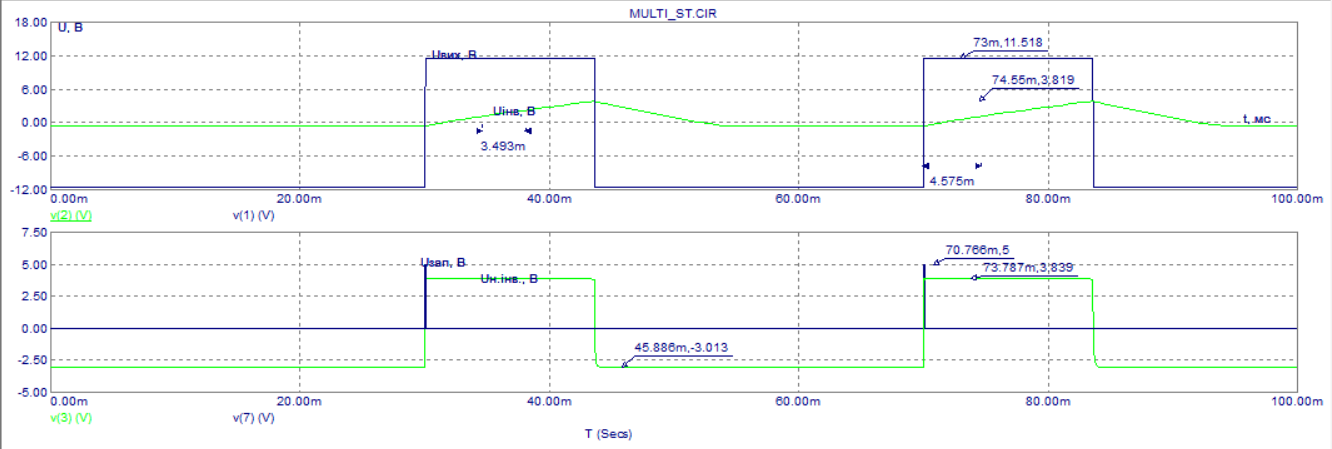
\includegraphics[width=1.1\textwidth]{diagrama 3.png}
        \caption{Часові діаграми роботи чекаючого мультивібратора}
    \end{figure}

    На часових діаграмах показано: на верхній осцилограмі — вихідну напругу ОП 
та напругу на інвертуючому вході (конденсатор $C_1$), на нижній — 
керувальний сигнал і напругу на неінвертуючому вході.

Після подачі живлення вихід ОП переходить у стан 
$U_{\text{вих}}=+U_{\text{нас}}$, а $U_{\text{зап}}=0$. Діод $D2$ при цьому 
закритий, і на неінвертуючому вході діє подільник $R_2 - R_4$:

\[
U_{n1} = \frac{U_{\max}}{R_2+R_4}R_2 = 3{,}83\text{ В}.
\]

Діод $D1$ також закритий, конденсатор $C_1$ заряджається до $U_{n1}$, після 
чого опорний рівень досягається і ОП перемикається у стан 
$U_{\text{вих}}=-U_{\text{нас}}$. У цьому режимі відкривається $D2$, тому:

\[
U_{n2} = -\frac{U_{\max}}{1+\frac{R_4}{R_2}} = -2{,}87\text{ В}.
\]

Після переходу $C_1$ перезаряджається. Якщо його напруга стає нижчою за 
$-U_{\text{D1,в}}$, відкривається $D1$ і фактично розряджає $C_1$. Таким 
чином схема переходить у стійкий стан, і без зовнішнього імпульсу вона не 
перемикається.

Пусковий імпульс подається через диференціюючий ланцюг $C_2$–$R_1$, і його 
тривалість:

\[
t_{\text{ім}} = R_5 C_1 \ln\!\left(1+\frac{R_2}{R_4}\right)
= 4.06\ \text{мс}.
\]

Час відновлення (перезаряд $C_1$):

\[
t_{\text{від}} = R_5 C_1 
\ln\!\left(1+\frac{2R_2}{R_4+R_2}\right) = 2.9\ \text{мс}.
\]

Для нормальної роботи період керувальних імпульсів має виконувати умову:
\[
t_{\text{пер}} > t_{\text{ім}} + t_{\text{від}}.
\]

    \newpage

    \begin{center} \textbf{\large Аналіз схеми №4} \end{center}

    \begin{figure}[h!]

        \renewcommand{\thefigure}{\arabic{figure}} % робимо "3.1", "3.2" і т.д.

        \centering
        \includegraphics[width=0.6\textwidth]{scheme4.pdf}
        % Підпис (зазвичай під малюнком):
        \caption{\centering Схема найпростішого ГЛЗН із зовнішнім запуском}
        % Мітка для посилань у тексті (\ref{fig:...})
        \label{fig2-1:schema}

    \end{figure}

    \begin{figure}[h!]

        \renewcommand{\thefigure}{\arabic{figure}} % робимо "3.1", "3.2" і т.д.

        \centering
        % Підставляєте потрібний шлях та розмір зображення:
       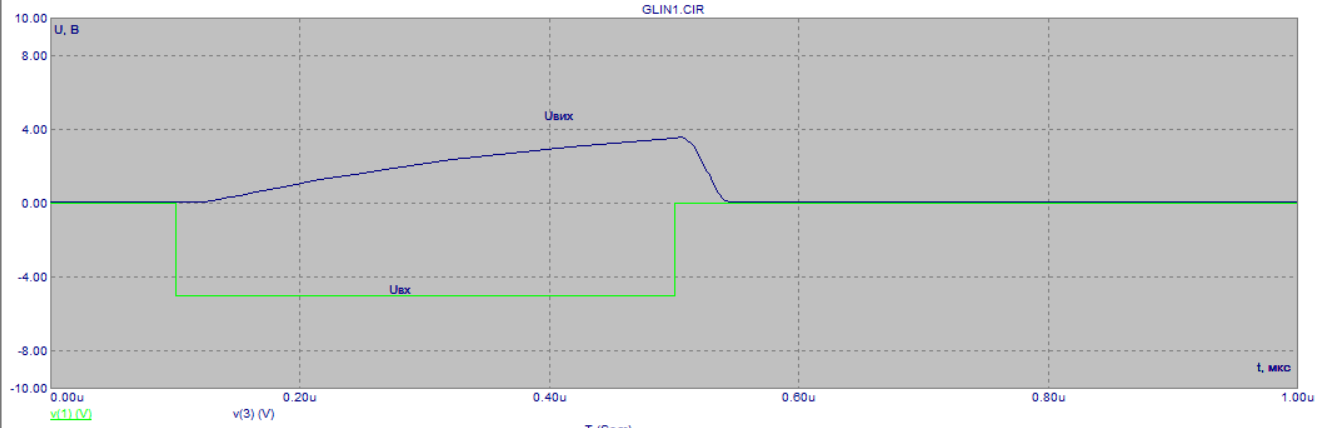
\includegraphics[width=1.1\textwidth]{diagrama 4.png}
        % Підпис (зазвичай під малюнком):
        \caption{Часові діаграми роботи для схеми}
        % Мітка для посилань у тексті (\ref{fig:...})
        \label{fig2-1:graph}

    \end{figure}

  Дана схема є транзисторним ключем з інтегруючим конденсатором $C_1$ на 
виході. У початковому стані транзистор $Q1$ відкритий, тому вихідна 
напруга формується джерелом $V2$ через резистор $R2$ і має невелике 
додатне значення.

Під час подачі від'ємного керувального імпульсу транзистор закривається, 
і конденсатор $C_1$ починає заряджатися від напруги $V2$ через резистор 
$R3$ за експоненціальним законом. На осцилограмі спостерігається плавне 
зростання вихідної напруги до значення $U_{\text{вих,max}}$.

Після завершення імпульсу транзистор знову відкривається, і конденсатор 
швидко розряджається майже до нуля. Максимальна амплітуда вихідного 
сигналу визначається тривалістю керувального імпульсу та сталою часу 
ланцюга $\tau = R_3 C_1$.

    \newpage

    \begin{center} \textbf{\large Аналіз схеми №5} \end{center}

    \begin{figure}[h!]

        \renewcommand{\thefigure}{\arabic{figure}} % робимо "3.1", "3.2" і т.д.

        \centering
        % Підставляєте потрібний шлях та розмір зображення:
       \includegraphics[width=0.6\textwidth]{scheme5.pdf}
        % Підпис (зазвичай під малюнком):
        \caption{\centering Схема чекаючого ГЛЗН}
        % Мітка для посилань у тексті (\ref{fig:...})
        \label{fig3-1:schema}

    \end{figure}

    \begin{figure}[h!]

        \renewcommand{\thefigure}{\arabic{figure}} % робимо "3.1", "3.2" і т.д.

        \centering
        % Підставляєте потрібний шлях та розмір зображення:
       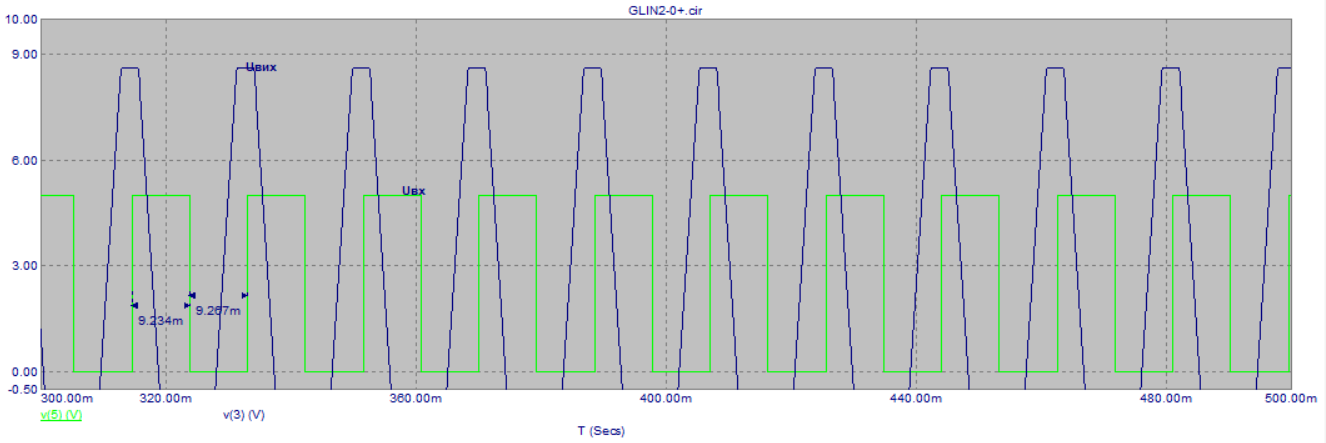
\includegraphics[width=1.1\textwidth]{diagrama 5-1.png}
       \caption{\centering Часові діаграми роботи схеми, яку наведено на рис, та в якій вихідний сигнал повинен змінюватися від 0 до +Uнас}
              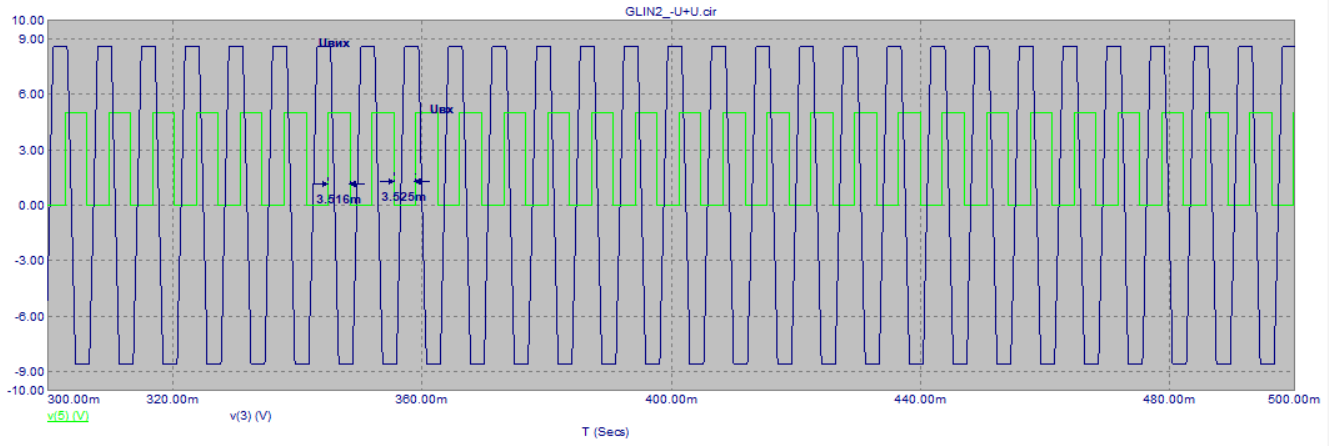
\includegraphics[width=1.1\textwidth]{diagrama 5-2.png}
        % Підпис (зазвичай під малюнком):
        \caption{\centering Часові діаграми роботи схеми, яку наведено на рис, та в якій вихідний сигнал повинен змінюватися від -Uнас до +Uнас}
        % Мітка для посилань у тексті (\ref{fig:...})
        \label{fig3-1:graph}

    \end{figure}

    \FloatBarrier

   На першій часовій діаграмі представлена робота схеми у режимі, в якому 
вихідна напруга змінюється в діапазоні від $0$ до $+U_{\text{нас}}$. 
У цьому випадку вихідний каскад формує лише додатні імпульси, а 
конденсатор $C_1$ заряджається до позитивного рівня, що визначає форму 
вихідного сигналу.

На другій часовій діаграмі показано режим, у якому вихідна напруга 
змінюється від $-U_{\text{нас}}$ до $+U_{\text{нас}}$. Тут операційний 
підсилювач працює симетрично, і конденсатор $C_1$ заряджається та 
розряджається в обох напрямках, що створює двополярні імпульси на виході.

Для отримання такого режиму схема моделювання залишається незмінною, але 
значення резисторів у керуючому ланцюгу приймаються рівними:
\[
R_1 = R_2 = 2~\text{k}\Omega.
\]
Такі значення забезпечують симетричну роботу діодів і дозволяють одержати 
вихідний сигнал у межах від $-U_{\text{нас}}$ до $+U_{\text{нас}}$.

    \begin{center} \textbf{\large Аналіз схеми №6} \end{center}

    \begin{figure}[h!]

        \renewcommand{\thefigure}{\arabic{figure}} % робимо "3.1", "3.2" і т.д.

        \centering
        % Підставляєте потрібний шлях та розмір зображення:
         \includegraphics[width=0.5\textwidth]{scheme6.pdf}
        % Підпис (зазвичай під малюнком):
        \caption{\centering Схема автоколивального ГЛЗН}
        % Мітка для посилань у тексті (\ref{fig:...})
        \label{fig4-1:schema}

    \end{figure}

    \begin{figure}[h!]

        \renewcommand{\thefigure}{\arabic{figure}} % робимо "3.1", "3.2" і т.д.

        \centering
        % Підставляєте потрібний шлях та розмір зображення:
       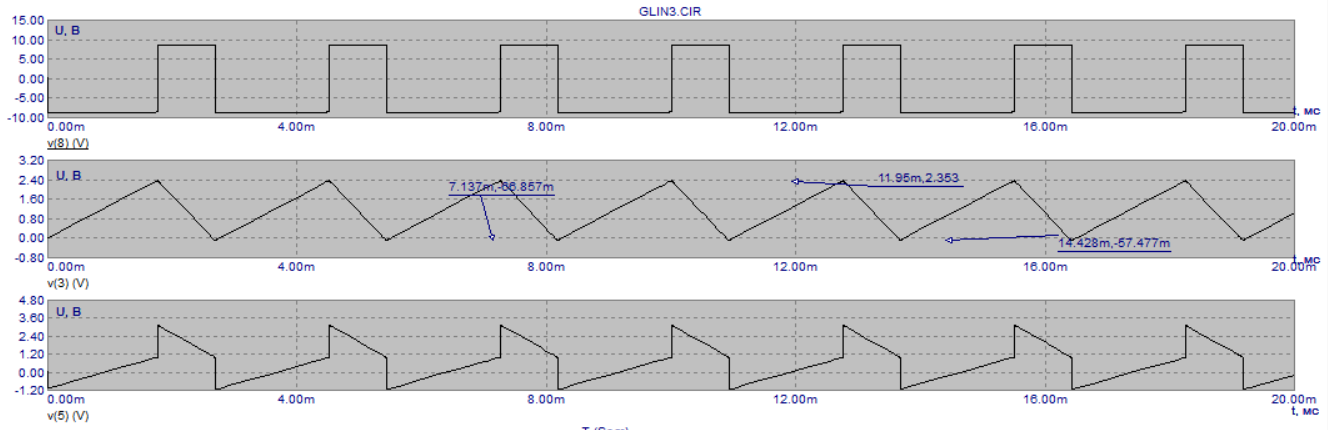
\includegraphics[width=1.1\textwidth]{diagrama 6.png}
        % Підпис (зазвичай під малюнком):
        \caption{\centering Часові діаграми роботи схеми}
        % Мітка для посилань у тексті (\ref{fig:...})
        \label{fig4-1:graph}

    \end{figure}
Перевіримо умову нормального функціонування генератора пили, яка задається 
співвідношенням:
\[
\frac{t_{\text{пр}}}{t_{\text{зв}}}=\frac{R_2}{R_1},
\]
де $t_{\text{пр}}$ — час прямого ходу пили (заряд конденсатора), 
а $t_{\text{зв}}$ — час зворотного ходу (розряд).

За часовою діаграмою отримуємо:
\[
t_{\text{пр}} \approx 7{,}14\ \text{мс}, \qquad
t_{\text{зв}} \approx 11{,}95\ \text{мс}.
\]

Підставимо у вираз:
\[
\frac{t_{\text{пр}}}{t_{\text{зв}}}
= \frac{7{,}14}{11{,}95} \approx 0{,}60,
\qquad
\frac{R_2}{R_1}
= \frac{20~\text{k}\Omega}{10~\text{k}\Omega} = 2.
\]

Як видно, умова нормальної роботи виконується приблизно: форма 
пилкоподібного сигналу відповідає очікуваному співвідношенню часу 
заряджання і розряджання, що визначається відношенням $R_2/R_1$.

    \vspace{1em}

    \noindent
    \textbf{\underline{Висновок:}} У ході роботи було досліджено принципи формування коливань у мультивібраторах та генераторах лінійно змінної напруги (ГЛЗН).
    Розглянуто їхні основні властивості, режими роботи, часові діаграми та вплив елементів схеми на форму сигналу. Також були проаналізовані ключові параметри цих пристроїв та визначено області їх практичного застосування у електронних генераторах, імпульсних схемах та формувачах сигналів.

\end{document}